\section{Lista 3: Algoritmos Recursivos} % <-----------------------------------------------------------------------------


\subsection{Algoritmo LMF} % <-----------------------------------------------------------------------------

O algoritmo é apresentado e debatido no trabalho \textit{The Least Mean Square Fourth (LMF) Algorithm
and Its Family} (Widrow, 1984), que foi utilizado de inspiração para solução desse problema.

Escrevendo a definição de erro em função do sinal desejado e da saída, obtemos:
\begin{align*}
    e(n) &= d(n) - y(n), \\
    e(n) &= d(n) - \mathbf{w}^{\text{T}}(n)\mathbf{x}(n),
\end{align*}

Utilizando o gradiente do erro elevado a quarta ordem, é possível obter a expressão de recursão através de derivação implícita:
\begin{align*}
    \nabla_{\mathbf{w}} \mathbb{E}\{e^{4}(n)\} &= \frac{\partial \mathbb{E}\{e^{4}(n)\}}{\partial \mathbf{w}} \\
    &= \mathbb{E} \left\{ \frac{\partial e^{4}(n)}{\partial \mathbf{w}}\right\} \\
    &= \mathbb{E}\left\{ \frac{\partial e^{4}(n)}{\partial e(n)} \cdot \frac{\partial e(n) }{\partial \mathbf{w}}\right\}
\end{align*}

Abrindo a expressão da derivação implícita, temos que:
\begin{align*}
    \nabla_{\mathbf{w}} \mathbb{E}\{e^{4}(n)\} &= \mathbb{E}\left\{4 e^{3}(n) \frac{\partial (d(n) - \mathbf{w}^{\text{T}}(n)\mathbf{x}(n)) }{\partial \mathbf{w}}\right\} \\
    &= \mathbb{E}\{4 e^{3}(n) (0 - \mathbf{x}(n))\} \\
    &= - 4 \mathbb{E}\{e^{3}(n) \mathbf{x}(n)\}
\end{align*}

Dado o resultado obtido em função de $\mathbb{E}\{e^{4}(n)\}$, visando minimizá-lo é necessário que $x(n)$ seja ortogonal à $e(n)$. Isto implica que:
\begin{align*}
    \mathbb{E}\{(d(n) - \mathbf{w}^{\text{T}}(n)\mathbf{x}(n))^{3} \mathbf{x}(n)\} = 0
\end{align*}

Ela permite demonstrar que a expressão converge em média, dado os seguintes parâmetros: $\sigma^{2}_{z}$ e $\lambda_{\text{max}}$, respectivamente, variância do ruído e o maior autovalor $\lambda_{\max}$ da matriz $\mathbf{R}_{x}$. Se o passo de aprendizado ($\mu_{\text{LMF}}$) for definido tal que:
\begin{align*}
    1 < \mu_{\text{LMF}} < \frac{1}{6 \sigma^{2}_{z} \lambda_{\text{max}}},
\end{align*}

O algoritmo recursivo do LMF é obtido a partir das expressões acima, reproduzindo a expressão semlhante ao do gradiente descendente, utilizando em problemas seguintes, de modo que:
\begin{align*}
    \mathbf{w}(n + 1) &= \mathbf{w}(n) - \mu_{\text{LMF}}\mathbf{g}_{w}(n) \\
    &= \mathbf{w}(n) + 4 \mu_{\text{LMF}} e^{3}(n) \mathbf{x}(n)
\end{align*}
\clearpage


\subsection{Algoritmo LMS} % <-----------------------------------------------------------------------------

\subsubsection*{Condição para convergência do algoritmo}

O erro nos coeficientes do filtro à cada iteração está associado à condição de convergência. Relacionando o erro dos coeficientes em um iteração qualquer com o filtro ótimo: $ \Delta \mathbf{w}(n) = \mathbf{w}(n) - \mathbf{w}_{\text{opt}} $. 

E isso permite aplicar a função de recurssão do LMS, de modo que:
\begin{align*}
    \Delta \mathbf{w}(n + 1) &= \Delta \mathbf{w}(n) + 2 \mu e(n) \mathbf{x}(n) \\
    &= \Delta \mathbf{w}(n) + 2 \mu \mathbf{x}(n) \left[e_{\text{opt}}(n) - \mathbf{x}^{\text{T}}(n) \Delta \mathbf{w}(n)\right] \\
    &= \left[ \mathbf{I} - 2 \mu \mathbf{x}(n) \mathbf{x}^{\text{T}}(n) \right] \Delta \mathbf{w}(n) + 2 \mu e_{\text{opt}}(n) \mathbf{x}(n)
\end{align*}

Aplicando o operador esperança em ambos os lados da expressão e reescrevendo o lado direito, partindo das relações $e(n) = e^{\text{T}}(n)$.
\begin{align*}
    \mathbb{E}\{\Delta \mathbf{w}(n + 1)\} &= \mathbb{E}\{\left[ \mathbf{I} - 2 \mu \mathbf{x}(n) \mathbf{x}^{\text{T}}(n) \right] \Delta \mathbf{w}(n) + 2 \mu e_{\text{opt}}(n) \mathbf{x}(n)\} \\
    &= \mathbb{E}\{\left[ \mathbf{I} - 2 \mu \mathbf{x}(n) \mathbf{x}^{\text{T}}(n) \right] \Delta \mathbf{w}(n)\} + 2 \mu \mathbb{E}\{e_{\text{opt}}(n) \mathbf{x}(n)\}
\end{align*}

Como em problemas anteriores, utilizamos novamente a vantagem do operador esperança ser um operador linear. Então, se temos simultaneamente que: $\mathbf{x}(n)$ é ortogonal a $e_{\text{opt}}(n)$ e $\Delta \mathbf{w}(n)$, logo:
\begin{align*}
    \mathbb{E}\{\Delta \mathbf{w}(n + 1)\} &= \left[ \mathbf{I} - 2 \mu \mathbb{E}\{\mathbf{x}(n) \mathbf{x}^{\text{T}}(n)\} \right] \mathbb{E}\{\Delta \mathbf{w}(n)\} \\
    &= \left( \mathbf{I} - 2 \mu \mathbf{R}_{x} \right) \mathbb{E}\{\Delta \mathbf{w}(n)\}
\end{align*}

Visando obter uma matriz diagonal para facilitar a análise de condicionamento do algoritmo, assume-se a existência uma matriz unitária que diagonaliza $\mathbf{R}_{x}$, $\mathbf{Q}$, onde:
\begin{align*}
    \mathbb{E}\{ \mathbf{Q}^{\text{T}} \Delta \mathbf{w}(n + 1) \} &= \left( \mathbf{I} - 2 \mu \mathbf{Q}^{\text{T}} \mathbf{R}_{x} \right) \mathbf{I} \mathbb{E}\{ \Delta \mathbf{w}(n)\} \\
    &= \left( \mathbf{I} - 2 \mu \mathbf{Q}^{\text{T}} \mathbf{R}_{x} \right) \mathbf{Q} \mathbf{Q}^{\text{T}} \mathbb{E}\{ \Delta \mathbf{w}(n)\} \\
    &= \left( \mathbf{I} - 2 \mu \mathbf{Q}^{\text{T}} \mathbf{R}_{x} \mathbf{Q} \right) \mathbb{E}\{ \mathbf{Q}^{\text{T}} \Delta \mathbf{w}(n)\} \\
\end{align*}

Reorganizando, tem-se que:
\begin{align*}
    \mathbb{E}\{\Delta \mathbf{w}'(n + 1)\} &= \left( \mathbf{I} - 2 \mu \mathbf{\Lambda} \right) \mathbb{E}\{\Delta \mathbf{w}'(n)\}
\end{align*}

A expressão anterior, pode ser expandida à esquerda para a análise de convergência do filtro, de modo que:
\begin{align*}
    \mathbb{E}\{ \Delta \mathbf{w}'(n + 1) \} &= \left( \mathbf{I} - 2 \mu \mathbf{\Lambda} \right)^{n + 1} \mathbb{E}\{\Delta \mathbf{w}'(0)\} \\
    &= \text{diag} \left[ (1 - 2 \mu \lambda_{1})^{n + 1}, (1 - 2 \mu \lambda_{2})^{n + 1}, \dots, (1 - 2 \mu \lambda_{N})^{n + 1}) \right] \mathbb{E}\{ \Delta \mathbf{w}'(0)\}
\end{align*}

Onde $\text{diag}(\cdot)$ é uma matriz diagonal contendo cada autovalor da matriz de autocorrelação, $\lambda_{n} \forall n \in \{1, \cdots, N\}$. Isso permite avaliar a condição de estabilidade apenas com propriedades relacionadas à $\lambda$. 

Finalmente, de acordo com a expressão anterior, temos que para garantir estabilidade na convergência, é necessário que o passo de aprendizado do algoritmo $\mu$ esteja contido entre $0$ e o maior autovalor. Desta forma é possível garantir que a medida que as dimensões dessa matriz aumenta, os valores vão reduzir, tendendo a zero:
\begin{align*}
    0 < \mu < \frac{1}{\lambda}_{\text{max}}
\end{align*}

\clearpage

\subsubsection*{Erro em excesso em média quadrática}
% \todo[inline, color=yellow!30]{Organizar}

% O erro em excesso é normalmente ocasionado pelos termos ruidosos presentes no gradiente, impedindo que os coeficientes convirjam de forma exata para a solução ótima. 
% Podemos iniciar essa análise escrevendo a equação para o erro de estimação para um determinado instante $n$ como se segue

% \begin{align*}
%     e(n) &= d(n) - \mathbf{w}^{\text{T}}_{\text{opt}} \mathbf{x}(n) - \Delta \mathbf{w}^{\text{T}}(n) \mathbf{x}(n), \\
%     e(n) &= e_{\text{opt}}(n) - \Delta \mathbf{w}^{\text{T}}(n) \mathbf{x}(n),
% \end{align*}

% onde o erro quadrático é expresso por

% \begin{align*}
%     e^{2}(n) &= e^{2}_{\text{opt}}(n) - 2 e_{\text{opt}}(n) \Delta \mathbf{w}^{\text{T}}(n) \mathbf{x}(n) + \Delta \mathbf{w}^{\text{T}}(n) \mathbf{x}(n) \mathbf{x}^{\text{T}}(n) \Delta \mathbf{w}(n) ,
% \end{align*}

% se definirmos o erro quadrático médio como $\xi(n) = \mathbb{E}\{e^{2}(n)\}$ e o erro ótimo, leia-se mínimo, como $\xi_{\text{min}} = \mathbb{E}\{e^{2}_{\text{opt}}(n)\}$
% então podemos escrever

% \begin{align*}
%     \xi(n) = \xi_{\text{min}} - 2 \mathbb{E}\{e_{\text{opt}}(n) \Delta \mathbf{w}^{\text{T}}(n) \mathbf{x}(n)\} + \mathbb{E}\{\Delta \mathbf{w}^{\text{T}}(n) \mathbf{x}(n) \mathbf{x}^{\text{T}}(n) \Delta \mathbf{w}(n)\},
% \end{align*}

% considerando mais uma vez que $\mathbf{x}$ é ortogonal ao $\Delta \mathbf{w}^{\text{T}}(n)$ e ao $e_{\text{opt}}(n)$, simultaneamente, podemos simplificar a expressão ainda mais 

% \begin{align*}
%     \xi(n) = \xi_{\text{min}} - 2 \mathbb{E}\{\Delta \mathbf{w}^{\text{T}}(n)\} \mathbb{E}\{e_{\text{opt}}(n) \mathbf{x}(n)\} + \mathbb{E}\{\Delta \mathbf{w}^{\text{T}}(n) \mathbf{x}(n) \mathbf{x}^{\text{T}}(n) \Delta \mathbf{w}(n)\},
% \end{align*}

% onde podemos utilizar a propriedade $\mathbb{E}\{\Delta \mathbf{w}^{\text{T}}(n) \mathbf{x}(n) \mathbf{x}^{\text{T}}(n) \Delta \mathbf{w}(n)\} = \text{tr}(\mathbb{E}\{\Delta \mathbf{w}^{\text{T}}(n) \mathbf{x}(n) \mathbf{x}^{\text{T}}(n) \Delta \mathbf{w}(n)\})$ uma vez
% que sabemos que o traço de um escalar é o próprio escalar. Sendo assim, utilizando a propriedade cíclica do operador traço escrevemos

% \begin{align*}
%     \xi(n) &= \xi_{\text{min}} - 2 \mathbb{E}\{\Delta \mathbf{w}^{\text{T}}(n)\} \mathbb{E}\{e_{\text{opt}}(n) \mathbf{x}(n)\} + \text{tr}(\mathbb{E}\{\Delta \mathbf{w}^{\text{T}}(n) \mathbf{x}(n) \mathbf{x}^{\text{T}}(n) \Delta \mathbf{w}(n)\}), \\
%     \xi(n) &= \xi_{\text{min}} - 2 \mathbb{E}\{\Delta \mathbf{w}^{\text{T}}(n)\} \mathbb{E}\{e_{\text{opt}}(n)\mathbf{x}(n)\} + \mathbb{E}\{\text{tr}[\Delta \mathbf{w}^{\text{T}}(n) \mathbf{x}(n) \mathbf{x}^{\text{T}}(n) \Delta \mathbf{w}(n)]\}, \\
%     \xi(n) &= \xi_{\text{min}} - 2 \mathbb{E}\{\Delta \mathbf{w}^{\text{T}}(n)\} \mathbb{E}\{e_{\text{opt}}(n)\mathbf{x}(n)\} + \mathbb{E}\{\text{tr}[\mathbf{x}(n) \mathbf{x}^{\text{T}}(n) \Delta \mathbf{w}(n) \Delta \mathbf{w}^{\text{T}}(n)]\}, \\
%     \xi(n) &= \xi_{\text{min}} + \mathbb{E}\{\text{tr}[\mathbf{x}(n) \mathbf{x}^{\text{T}}(n) \Delta \mathbf{w}(n) \Delta \mathbf{w}^{\text{T}}(n)]\}, \\
%     \xi(n) &= \xi_{\text{min}} + \text{tr}(\mathbb{E}\{\mathbf{x}(n) \mathbf{x}^{\text{T}}(n) \Delta \mathbf{w}(n) \Delta \mathbf{w}^{\text{T}}(n)\}), \\
%     \xi(n) &= \xi_{\text{min}} + \text{tr}(\mathbb{E}\{\mathbf{x}(n) \mathbf{x}^{\text{T}}(n)\} \mathbb{E}\{\Delta \mathbf{w}(n) \Delta \mathbf{w}^{\text{T}}(n)\}), \\
%     \xi(n) &= \xi_{\text{min}} + \text{tr}(\mathbf{R}_{x} \mathbb{E}\{\Delta \mathbf{w}(n) \Delta \mathbf{w}^{\text{T}}(n)\}), \\
%     \xi(n) &= \xi_{\text{min}} + \text{tr}(\mathbb{E}\{\mathbf{R}_{x} \Delta \mathbf{w}(n) \Delta \mathbf{w}^{\text{T}}(n)\}), 
% \end{align*}

% onde o processo justifica-se pela intercambialidade entre os operadores traço e valor esperador e pela ortogonalidade mencionada anteriormente. Em sequência podemos definir o erro em excesso por

% \begin{align}
%     \xi(n) - \xi_{\text{min}} &= \text{tr}(\mathbb{E}\{\mathbf{R}_{x} \Delta \mathbf{w}(n) \Delta \mathbf{w}^{\text{T}}(n)\}), \\
%     \Delta \xi(n) &= \text{tr}(\mathbb{E}\{\mathbf{R}_{x} \Delta \mathbf{w}(n) \Delta \mathbf{w}^{\text{T}}(n)\}), \label{excesso1}
% \end{align}

% e adicionalmente, pela definição de uma transformação de similaridade onde garantimos que exista $\mathbf{Q} \mathbf{Q}^{\text{T}} = \mathbf{I}$ capaz de diagonalizar a matriz de autocorrelação, podemos reescrever a Equação (\ref{excesso1}) da seguinte forma

% \begin{align}
%     \Delta \xi(n) &= \text{tr}(\mathbb{E}\{\mathbf{Q} \mathbf{Q}^{\text{T}} \mathbf{R}_{x} \mathbf{Q} \mathbf{Q}^{\text{T}} \Delta \mathbf{w}(n) \Delta \mathbf{w}^{\text{T}}(n) \mathbf{Q} \mathbf{Q}^{\text{T}}\}), \\
%     \Delta \xi(n) &= \text{tr}(\mathbb{E}\{\mathbf{Q} \mathbf{\Lambda} \mathbf{Q}^{\text{T}} \Delta \mathbf{w}(n) \Delta \mathbf{w}^{\text{T}}(n) \mathbf{Q} \mathbf{Q}^{\text{T}}\}), \\
%     \Delta \xi(n) &= \text{tr}(\mathbb{E}\{\mathbf{Q} \mathbf{\Lambda} \text{cov} \left[\Delta \mathbf{w}'(n)\right] \mathbf{Q}^{\text{T}}\}), \\
%     \Delta \xi(n) &= \text{tr}(\mathbb{E}\{\mathbf{\Lambda} \text{cov} \left[\Delta \mathbf{w}'(n)\right] \mathbf{Q}^{\text{T}} \mathbf{Q}\}), \\
%     \Delta \xi(n) &= \text{tr}(\mathbb{E}\{\mathbf{\Lambda} \text{cov} \left[\Delta \mathbf{w}'(n)\right]\}), \label{excesso2}
% \end{align}

% onde é sabido que $\text{cov} \left[\Delta \mathbf{w}(n)\right] = \mathbb{E}\{(\mathbf{w}(n) - \mathbf{w}_{\text{opt}}) (\mathbf{w}(n) - \mathbf{w}_{\text{opt}})^{\text{T}}\}$ e $\Delta \mathbf{w}'(n) = \mathbf{Q}^{\text{T}} \Delta \mathbf{w}(n) \Delta \mathbf{w}^{\text{T}}(n) \mathbf{Q}$.
% Enfim, a partir das orientações presentes no livro texto da disciplina a respeito da matriz de covariância do vetor de erros é possível ainda escrever a Equação (\ref{excesso2}) como

% \begin{align*}
%     \Delta \xi(n) &= \sum^{N}_{i = 1} \lambda_{i} v_{i}'(n) = \mathbf{\lambda}^{\text{T}} \mathbf{v}'(n),
% \end{align*}

% onde $\mathbf{\lambda}$ é um vetor contendo todos os autovalores da matriz de autocorrelação e $\mathbf{v}(n)$ é um vetor que contém os elementos da diagonal de $\text{cov} \left[\Delta \mathbf{w}'(n)\right]$. Em suma, podemos 
% expressar o $i$th elemento do vetor diagonal $\mathbf{v}'(n + 1)$, seguindo orientações disponíveis no livro texto da disciplina, com o seguinte equacionamento

% \begin{align*}
%     v_{i}'(n + 1) &= (1 - 4 \mu \lambda_{i} + 8 \mu^{2} \lambda^{2}_{i}) v_{i}'(n) + 4 \mu^{2} \lambda_{i} \sum^{N}_{j = 0} \lambda_{j} v_{j}'(n) + 4 \mu^{2} \sigma^{2}_{z} \lambda_{i}.
% \end{align*}

% Entretanto, se considerarmos que $v_{i}'(n + 1) \approx v_{i}'(n)$ quando $n \rightarrow \infty$ podemos simplificar a expressão, além de que 
% também podemos realizar uma operação de soma total dos parâmetros para obter o erro em excesso total

% \begin{align*}
%     \notag &\sum^{N}_{i = 1} v_{i}'(n) = \sum^{N}_{i = 1} (1 - 4 \mu \lambda_{i} + 8 \mu^{2} \lambda^{2}_{i}) v_{i}'(n) + 4 \mu^{2} \sum^{N}_{i = 1} \lambda_{i} \sum^{N}_{j = 0} \lambda_{j} v_{j}'(n) + 4 \mu^{2} \sigma^{2}_{z} \sum^{N}_{i = 1} \lambda_{i}, \\
%     \notag &\sum^{N}_{i = 1} v_{i}'(n) = \sum^{N}_{i = 1} v_{i}'(n) - 4 \mu \sum^{N}_{i = 1} \lambda_{i} v_{i}'(n)  + 8 \mu^{2} \sum^{N}_{i = 1} \lambda^{2}_{i} v_{i}'(n) + 4 \mu^{2} \sum^{N}_{i = 1} \lambda_{i} \sum^{N}_{j = 0} \lambda_{j} v_{j}'(n) + 4 \mu^{2} \sigma^{2}_{z} \sum^{N}_{i = 1} \lambda_{i}, \\
%     \notag &\sum^{N}_{i = 1} v_{i}'(n) - \sum^{N}_{i = 1} v_{i}'(n) + 4 \mu \sum^{N}_{i = 1} \lambda_{i} v_{i}'(n) - 4 \mu^{2} \sum^{N}_{i = 1} \lambda_{i} \sum^{N}_{j = 0} \lambda_{j} v_{j}'(n) = 4 \mu^{2} \sigma^{2}_{z} \sum^{N}_{i = 1} \lambda_{i} + 8 \mu^{2} \sum^{N}_{i = 1} \lambda^{2}_{i} v_{i}'(n), \\
%     \notag &4 \mu \sum^{N}_{j = 1} \lambda_{j} v_{j}'(n)(1 - \mu \sum^{N}_{i = 1} \lambda_{i}) = 4 \mu (\mu \sigma^{2}_{z} \sum^{N}_{i = 1} \lambda_{i} + 2 \mu \sum^{N}_{i = 1} \lambda^{2}_{i} v_{i}'(n)), \\
%     \notag &\sum^{N}_{j = 1} \lambda_{j} v_{j}'(n) = \frac{\mu \sigma^{2}_{z} \sum^{N}_{i = 1} \lambda_{i} + 2 \mu \sum^{N}_{i = 1} \lambda^{2}_{i} v_{i}'(n)}{1 - \mu \sum^{N}_{i = 1} \lambda_{i}}, \\
%     \notag &\sum^{N}_{j = 1} \lambda_{j} v_{j}'(n) \approx \frac{\mu \sigma^{2}_{z} \sum^{N}_{i = 1} \lambda_{i} }{1 - \mu \sum^{N}_{i = 1} \lambda_{i}}, \\
%     &\sum^{N}_{j = 1} \lambda_{j} v_{j}'(n) = \frac{\mu \sigma^{2}_{z} \text{tr}(\mathbf{R}_{x})}{1 - \mu \text{tr}(\mathbf{R}_{x})},
% \end{align*}

% onde foi considerado que o termo $2 \mu \sum^{N}_{i = 1} \lambda^{2}_{i} v_{i}'(n)$ apresenta contribuição insignificante para o valor absoluto do numerador. Entretanto, é mencionado no livro texto que tal aproximação é de prova complexa, mas que normalmente 
% se verifica verdadeira para pequenos valores do passo de aprendizado $\mu$. Portanto, o erro em excesso pode ser prontamente descrito pela expressão que se segue

% \begin{align*}
%     \xi_{\text{excesso}} &= \underset{n \rightarrow \infty}{\text{lim}} \Delta \xi(n) \approx \frac{\mu \sigma^{2}_{z} \text{tr}(\mathbf{R}_{x})}{1 - \mu \text{tr}(\mathbf{R}_{x})}.
% \end{align*}

% Vale ainda expor que podemos considerar $1 - \mu \text{tr}(\mathbf{R}_{x}) \approx 1$ para valores muito pequenos de $\mu$, obtendo assim uma versão aproximada para o erro em excesso dada por

% \begin{align*}
%     \xi_{\text{excesso}} &= \underset{n \rightarrow \infty}{\text{lim}} \Delta \xi(n) \approx \mu \sigma^{2}_{z} \text{tr}(\mathbf{R}_{x}).
% \end{align*}

% \clearpage


\subsection{Algoritmo LMS Normalizado} % <-----------------------------------------------------------------------------
A expressão recursiva do algoritmo NLMS para atualização dos coeficientes de filtro é dada por:
\begin{align*}
    \mathbf{w}(k+1) = \mathbf{w}(k) + \frac{\mu_{norm}}{\gamma + \mathbf{x}^{\text{T}}(k) \mathbf{x}(k)} \mathbf{e}(k) \mathbf{x}(k),
\end{align*}

A partir da relação com o algortimo LMS, asssumindo um valor médio de $\mu$, na direção de $2 \mathbf{e}(k) \mathbf{x}(k)$ está diretamente relacionado com a expressão: 
\begin{align*}
    \frac{\mu_{norm}}{2 \text{trace}(\mathbf{R_{xx}})}
\end{align*}

Finalmente, isso permite limitar à direita o valor de convergência do NLMS, tendo como parâmetro as equações utilizadas na atualização do LMS.
\begin{align*}
    0 &< \frac{\mu_{norm}}{2 \text{trace}(\mathbf{R_{xx}})} < \frac{1}{\text{trace}(\mathbf{R_{xx}})} \\
    0 &< \mu_{norm} < 2, 
\end{align*}
        

\subsection{Equalização de Canais} % <-----------------------------------------------------------------------------

\subsubsection*{Equalizado Ótimo e plano Z}

Considerando o sinal gaussiano branco $x(n)$, a saída do canal $y(n)$ é dada por: $ y(n) = x(n) + 1.6 x(n - 1)$. Consequentemente, tem a seguinte a matriz de autocorrelação:
\begin{align*}
    \mathbf{R}_{y} =
    \begin{bmatrix}
        \mathbb{E}\{y(n)y^{\text{H}}(n)\} & \mathbb{E}\{y(n)y^{\text{H}}(n - 1)\} \\
        \mathbb{E}\{y(n - 1)y^{\text{H}}(n)\} & \mathbb{E}\{y(n - 1)y^{\text{H}}(n - 1)\}
    \end{bmatrix},
\end{align*}

Aplicando os valores em cada expressão de correlação, e sabendo que sinal tem média nula e suas amostras são independentes, temos que matriz de autocorrelação teórica:
\begin{align*}
    \mathbf{R}_{y} =
    \begin{bmatrix}
        3.56 & 1.60 \\
        1.60 & 3.56
    \end{bmatrix}
\end{align*}

O vetor de correlação cruzada é dado por:
\begin{align*}
    \mathbf{p}_{yd} =
    \begin{bmatrix}
        \mathbb{E}\{y(n)d(n)\} \\
        \mathbb{E}\{y(n - 1)d(n)\}
    \end{bmatrix} = 
    \begin{bmatrix}
        1 \\
        0
    \end{bmatrix},
\end{align*}
buscando obter a maior correlação possivel com o sinal desejado, sem que haja dependência de amostras em instantes diferentes. Por fim, temos que os coeficientes ótimos (Wiener) do equalizador são:
\begin{align*}
    \mathbf{w}_{\text{opt}} &= \mathbf{R}^{-1}_{y} \mathbf{p}_{yd} \\
    &= \begin{bmatrix}
        0.35 &  -0.16 \\
        -0.16 & 0.35
    \end{bmatrix} 
    \begin{bmatrix}
        1 \\
        0
    \end{bmatrix} \\
    &= \begin{bmatrix}
        0.35 \\
        -0.16
    \end{bmatrix} 
\end{align*}

\begin{figure}[!htp]
    \centering
    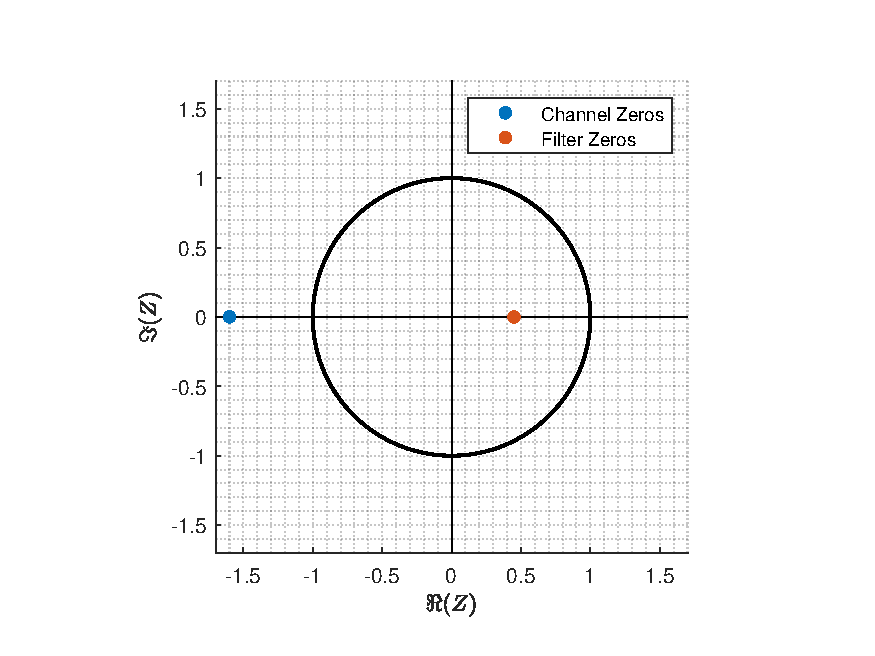
\includegraphics[width=0.8\textwidth]{fig/hw3p4-zeros.pdf}
    \caption{Zeros do canal e do equalizador no plano-z.}
    \label{fig:hw3p4-zeros}
\end{figure}

Levando em consideração todas as informações obtidas, é possível calculcar o diagram de zeros do filtro e do canal na Fig.~\ref{fig:hw3p4-zeros}.

\subsubsection*{Filtro de Erro de Predição Direta de Passo Unitário}
O filtro de predição direta de passo unitário é dado por:
\begin{align*}
    \hat{x}(n) &= \sum^{M + k - 1}_{i = k} w_{f,i} x(n - i) \\
    &= \sum^{2}_{i = 1} w_{f,i} x(n - i) \\
    &= \mathbf{w}^{\text{T}}_{f} \mathbf{x}(n - 1),
\end{align*}

Tendo que o erro quadrático médio (MSE) é:
\begin{align*}
    \mathbb{E}\{e^{2}(n)\} &= \mathbb{E}\{(x(n) - \hat{x}(n) )^{2}\} \\
    &= \mathbf{r}_{x}(0) - 2 \mathbf{w}^{\text{T}}_{f} \mathbf{r}_{x,f} + \mathbf{w}^{\text{T}}_{f} \mathbf{R}_{x} \mathbf{w}_{f}
\end{align*}
E a solução ótima é: $ \mathbf{w}_{f,\text{opt}} = \mathbf{R}^{-1}_{x} \mathbf{r}_{x,f} $.

Teremos assim que a mesma matriz de autocorrelação e o vetor de correlação cruzada serão definidos por
\begin{align*}
    \mathbf{r}_{y,f} &= 
    \begin{bmatrix}
        r_{y}(1) \\
        r_{y}(2)
    \end{bmatrix} \\
    & =
    \begin{bmatrix}
        \mathbb{E}\{y(n) y(n - 1)\} \\
        \mathbb{E}\{y(n) y(n - 2)\}
    \end{bmatrix} \\
    & = 
    \begin{bmatrix}
        1.60 \\
        0
    \end{bmatrix}.
\end{align*}

Logo, os coeficientes do filtro são:
\begin{align*}
    \mathbf{w}_{f,\text{opt}} &= 
    \begin{bmatrix}
        0.35 & -0.16 \\
        -0.16 & 0.35
    \end{bmatrix}
    \begin{bmatrix}
        1.60 \\
        0
    \end{bmatrix} \\ 
    &=
    \begin{bmatrix}
        0.56 \\
        -0.26
    \end{bmatrix}.
\end{align*}

Por fim, podemos verificar o ponto de zero do filtro, como antecipado no Fig.~\ref{fig:hw3p4-zeros}, $ W(z) = 0.56 - 0.26 z^{-1}$:
\begin{align*}
    0.56 - 0.26 z^{-1} &= 0 \\
    z &= 0.45
\end{align*}

\subsubsection*{Curvas de MSE e de Nível dos algoritmos}

Como apresentado anteriormente, na seção 2, questão 5, o conceito de superfície de erro utilizado para traçar as curvas de nível e MSE é baseado respectivamente nas funções $J(w) = \sigma^{2}_{d} - 2\mathbf{w}^{\top}\mathbf{p}_{\mathbf{X} d} + w^{\top}\mathbf{R}_{X}\mathbf{w} $ e $J(w) = \mathbb{E}\{e^{2}(n)\}$.

\begin{figure}[!htp]
    \centering
    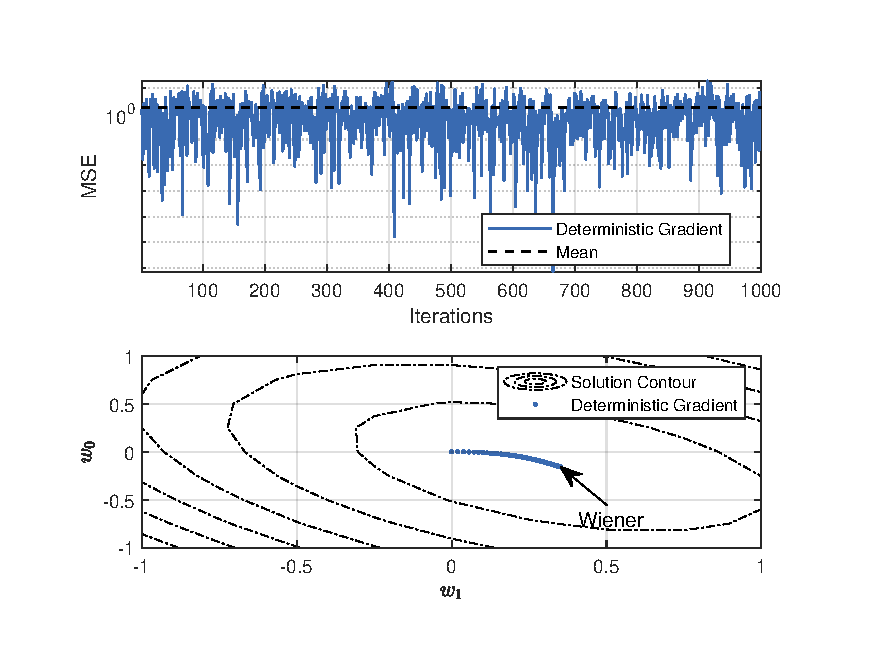
\includegraphics[width=0.80\textwidth]{fig/hw3p4-dga.pdf}
    \caption{Resultados da implementação do algoritmo gradiente determinístico com $N = 1000$ amostras, filtro de ordem $M = 2$ e parâmtro $\mu = 10^{-2}$. \textbf{Superior:} Evoulação da curva MSE. \textbf{Inferior:} Caminho percorrido até o ponto de convergência, i.e, filtro de Wiener.}
    \label{fig:hw3p4-dga}
\end{figure}

\begin{figure}[!htp]
    \centering
    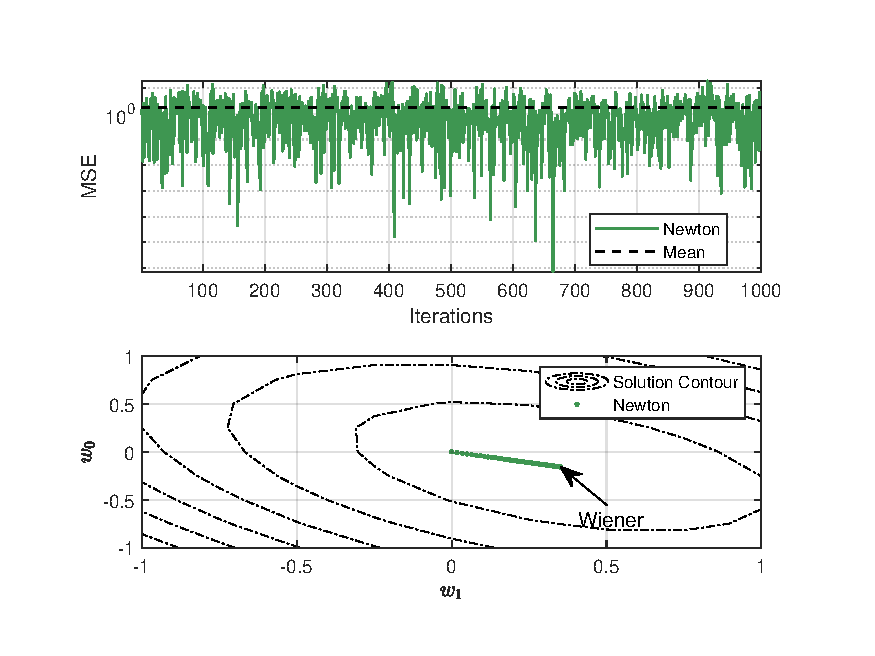
\includegraphics[width=0.80\textwidth]{fig/hw3p4-newton.pdf}
    \caption{Resultados da implementação do algoritmo Newton com $N = 1000$ amostras, filtro de ordem $M = 2$ e parâmtro $\mu = 0.5 \times 10^{-2}$. \textbf{Superior:} Evoulação da curva MSE. \textbf{Inferior:} Caminho percorrido até o ponto de convergência, i.e, filtro de Wiener.}
    \label{fig:hw3p4-newton}
\end{figure}

\begin{figure}[!htp]
    \centering
    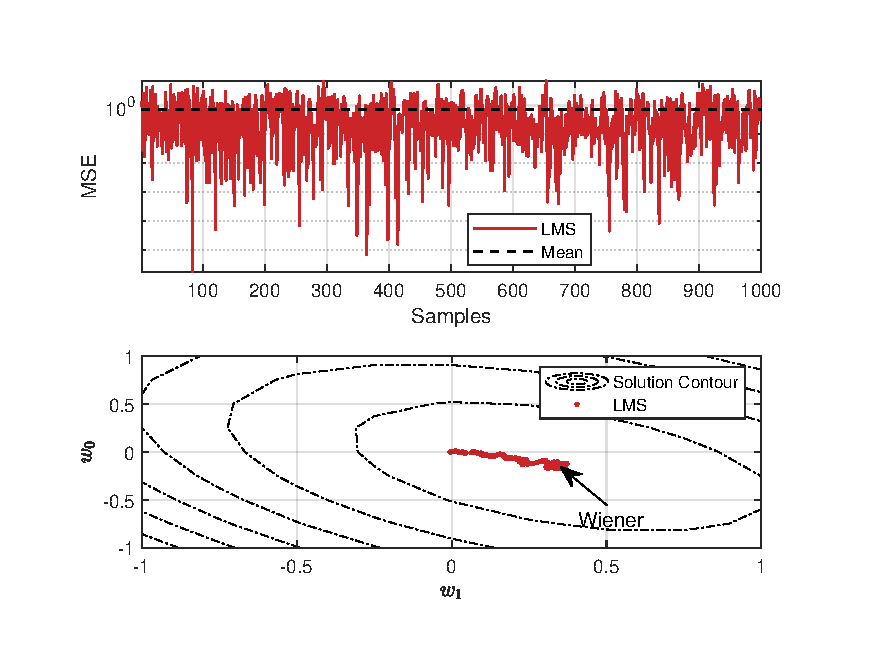
\includegraphics[width=0.80\textwidth]{fig/hw3p4-lms.pdf}
    \caption{Resultados da implementação do algoritmo LMS com $N = 1000$ amostras, filtro de ordem $M = 2$ e parâmtro $\mu = 10^{-3}$. \textbf{Superior:} Evoulação da curva MSE. \textbf{Inferior:} Caminho percorrido até o ponto de convergência, i.e, filtro de Wiener.}
    \label{fig:hw3p4-lms}
\end{figure}

\begin{figure}[!htp]
    \centering
    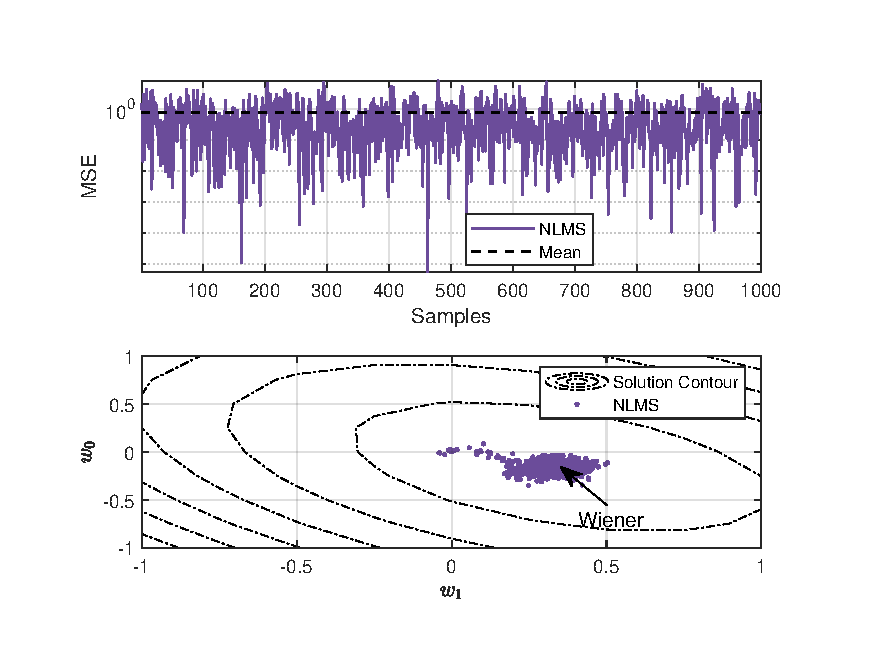
\includegraphics[width=0.80\textwidth]{fig/hw3p4-nlms.pdf}
    \caption{Resultados da implementação do algoritmo NLMS com $N = 1000$ amostras, filtro de ordem $M = 2$ e parâmtros $\mu = 0.5 \times 10^{-1}$ and $\gamma = 0.5 $. \textbf{Superior:} Evoulação da curva MSE. \textbf{Inferior:} Caminho percorrido até o ponto de convergência, i.e, filtro de Wiener.}
    \label{fig:hw3p4-nlms}
\end{figure}


As Figuras \ref{fig:hw3p4-dga}, \ref{fig:hw3p4-newton}, \ref{fig:hw3p4-lms} e \ref{fig:hw3p4-nlms} apresentam o comportamento do erro quadrático médio (MSE) e as curvas de convergência sobre a superfície MSE para cada algoritmo implementado. A ordem de $M = 2$ foi utilizada para todos os filtros, consequentemente o vetor de pesos na atualização possui apenas 2 coeficientes atualizados por iteração. O desempenho médio é semelhante, com certa vantagem para o NLMS.

Para os métodos determinísticos, é possível observar que há convergência organizada e suave. Isso é esperado, dado que o algoritmo utiliza o conhecimento dos coeficientes ideais do filtro. Enquanto para os métodos estocásticos, é visível algumas regiões de desordem na convergência, isso é dado como consequência da utilização das aproximações estatísticas instantâneas do sinal para o cálculo dos coeficientes. Ao comparar o LMS e sua versão normalizada, o primeiro apresenta uma maior estabilidade de convergência, enquanto o segundo apresentar uma numvem de pontos bem menos densa em torno da solução de Wiener, além de pontos que aparentemente se afastam da solução, consequência das iterações iniciais.

\subsubsection*{Número de condicionamento}
O número de condicionamento consiste no quociente entre o maior $\lambda_{\max}$ e menor $\lambda_{\min}$ autovalor da matrix $\mathbf{R}_{x}$.

A partir da equação $\lambda^{2} - 7.12 \lambda + 10.11 = 0$, obtém-se as raízes do polinômio e consequentemente os autovalores e autovetores da matriz.

Utilizando o MATLAB para calcular o quociente entre autovalores máximo e mínimo, obtemos que:
\begin{align*}
    \mathbb{C} (\mathbf{R}_{x}) = \frac{5.160}{1.960} = 2.633
\end{align*}

\subsubsection*{Modelo de canal para número de condicionamento menor/maior que 5}

Definindo uma função de transferência do canal: $H(z) = a_{0} + a_{1}z^{-1}$, pode-se obter a matriz de autocorrelação, visando obter o polinômio característico: $\lambda^{2} + b \lambda + c = 0$.
\begin{align*}
    \mathbf{R}_{y} =
    \begin{bmatrix}
        a_{0} + a^{2}_{1} & a_{1}\\
        a_{1} & a_{0} + a^{2}_{1}
    \end{bmatrix},
\end{align*}

Reorganizando a equação característica obtida a partir da matriz, tem-se que:
\begin{align*}
    &\lambda^{2} \overbrace{- 2 (a_{0} + a^{2}_{1})}^{b} \lambda + \overbrace{(a_{0} + a^{2}_{1})^{2} - a^{2}_{1}}^{c} = 0 \\
    &\lambda^{2} + b \lambda + c = 0
\end{align*}

A solução de equação de 2º grau pode ser obtida através equação de Bháskara, de modo que:

\begin{align*}
    \mathbb{C} (\mathbf{R}_{x}) &= \frac{\lambda_{\text{max}}}{\lambda_{\text{min}}} \\
     &= \frac{2 (a_{0} + a^{2}_{1}) + \sqrt{4 (a_{0} + a^{2}_{1})^{2} - 4 (a_{0} + a^{2}_{1})^{2} + 4 a^{2}_{1}}}{2 (a_{0} + a^{2}_{1}) - \sqrt{4 (a_{0} + a^{2}_{1})^{2} - 4 (a_{0} + a^{2}_{1})^{2} + 4 a^{2}_{1}}} \\
     &= \frac{a_{0} + a^{2}_{1} + a_{1}}{a_{0} + a^{2}_{1} - a_{1}}
\end{align*}

As relações acima permitem estabelecer as inequações que limitam o número de condicionamento: $ 5 (a_{0} + a^{2}_{1} - a_{1}) \leq a_{0} + a^{2}_{1} + a_{1} \leq 5 (a_{0} + a^{2}_{1} - a_{1})$.

% \clearpage


\subsection{Identificação de Sistemas} % <-----------------------------------------------------------------------------

\subsubsection*{Limite Superior para $\mu$}

Para definir o limite superior do fator de aprendizado, i.e, assegurar estabilidade, é necessário obter $\lambda_{\max}$ de $R_X$. 

Para isso é necessário desenvolver as equações que caracterizam o sistema, função de transferência e a representação da saída no tempo, respectivamente:
\begin{align*}
    H(z) &= \frac{1 - z^{-12}}{1 - z^{-1}} \\
    &= \frac{(1 - z^{-1})(\sum_{k= 0}^{11} z^{-k})}{1 - z^{-1}} \\
    &= \sum_{k = 0}^{11} z^{-k}
\end{align*}
\begin{align*}
    y(n) = \sum_{k = 0}^{11} x(n-k)
\end{align*}

Tendo essas informações, é possível estimar a $R_X$ utilizando o MATLAB, mostrada na Tabela ~\ref{tab:rxx}.
\begin{table}[!htb]
    \centering
    \begin{tabular}{llllllllllll}
    11.9509 & 10.9518 & 9.9530  & 8.9546  & 7.9567  & 6.9589  & $\dots$ & 0.9785  \\
    10.9518 & 11.9509 & 10.9518 & 9.9530  & 8.9546  & 7.9567  & $\dots$ & 1.9749  \\
    9.9530  & 10.9518 & 11.9509 & 10.9518 & 9.9530  & 8.9546  & $\dots$ & 2.9716  \\
    8.9546  & 9.9530  & 10.9518 & 11.9509 & 10.9518 & 9.9530  & $\dots$ & 3.9684  \\
    7.9567  & 8.9546  & 9.9530  & 10.9518 & 11.9509 & 10.9518 & $\dots$ & 4.9654  \\
    6.9589  & 7.9567  & 8.9546  & 9.9530  & 10.9518 & 11.9509 & $\dots$ & 5.9620  \\
    5.9620  & 6.9589  & 7.9567  & 8.9546  & 9.9530  & 10.9518 & $\dots$ & 6.9589  \\
    4.9654  & 5.9620  & 6.9589  & 7.9567  & 8.9546  & 9.9530  & $\dots$ & 7.9567  \\
    3.9684  & 4.9654  & 5.9620  & 6.9589  & 7.9567  & 8.9546  & $\dots$ & 8.9546  \\
    2.9716  & 3.9684  & 4.9654  & 5.9620  & 6.9589  & 7.9567  & $\dots$ & 9.9530  \\
    1.9749  & 2.9716  & 3.9684  & 4.9654  & 5.9620  & 6.9589  & $\dots$ & 10.9518 \\
    0.9785  & 1.9749  & 2.9716  & 3.9684  & 4.9654  & 5.9620  & $\dots$ & 11.9509
    \end{tabular}
    \caption{Matriz de autocorrelação $R_X$, com simulação de Monte Carlo, utilizando 10000 iterações.}
    \label{tab:rxx}
\end{table}

De acordo com o autovalor máximo, obtido no MATLAB, temos o seguinte intervalo de convergência:
\begin{align*}
    0 < \mu < \frac{1}{97}
\end{align*}

\subsubsection*{O algoritmo para $\frac{\mu_{\text{max}}}{2}$, $\frac{\mu_{\text{max}}}{10}$ e $\frac{\mu_{\text{max}}}{50}$} 


As Figuras~\ref{fig:mu_2}, \ref{fig:mu_10} e \ref{fig:mu_50} mostram o desempenho de cada filtro, de acordo com os parâmetros, e o apresentam o comportamento dos coeficientes na convergência do algoritmo. 

A primeira vista, o rastreio do resposta em frequência é o que deixa mais evidente a relação entre a diminuição do $\mu$ e a piora do desempenho. Isso se dá, pois ao passo que o $\mu$ reduz-se, a flexibilidade de adaptação diminui concomitantemente, tornando mais difícil do filtro acompanhar mudanças no canal.

\begin{figure}[!htp]
    \centering
    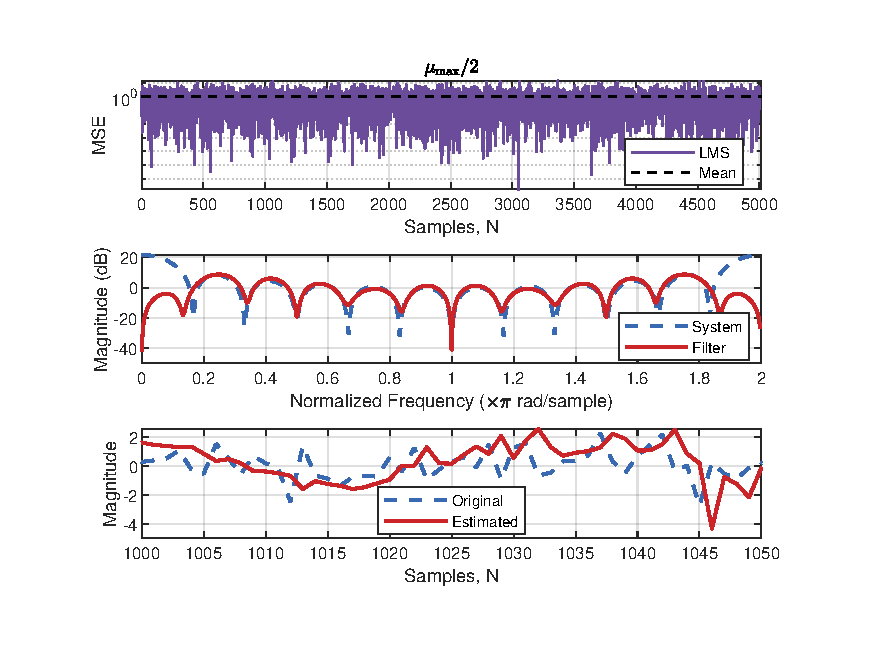
\includegraphics[width=0.9\textwidth]{C:/Users/lucasabdalah-dell/Documents/GitHub/Courses-HWs/Master/TIP7188-FILTRAGEM_ADAPTATIVA/homework/code/figures/hw3p5b-mu02.pdf}
    \caption{$\text{Amostras} = 5000$, $M = 15$, $\mu = \frac{\mu_{\text{max}}}{2}$}
    \label{fig:mu_2}
\end{figure}

\begin{figure}[!htp]
    \centering
    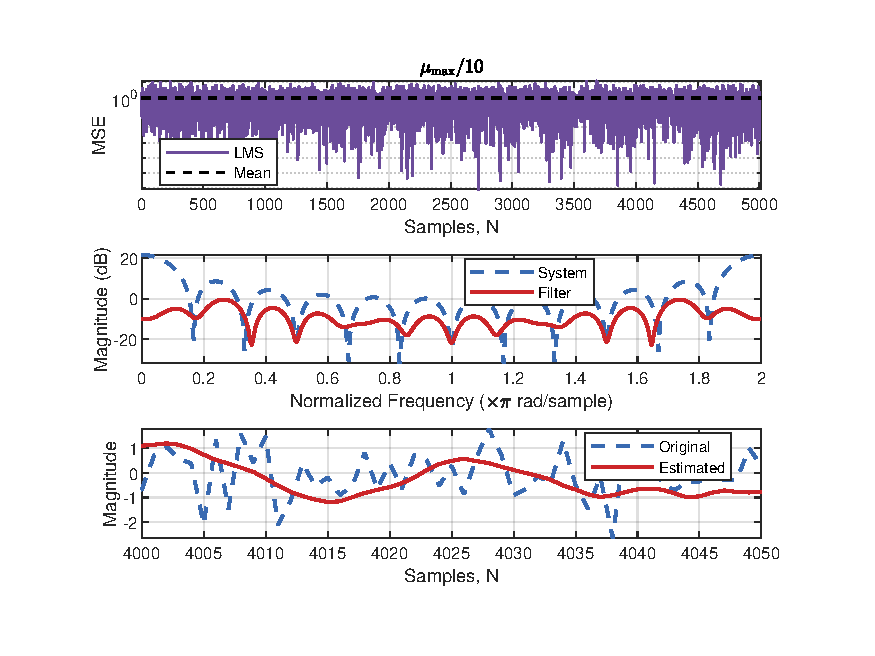
\includegraphics[width=0.9\textwidth]{C:/Users/lucasabdalah-dell/Documents/GitHub/Courses-HWs/Master/TIP7188-FILTRAGEM_ADAPTATIVA/homework/code/figures/hw3p5b-mu10.pdf}
    \caption{$\text{Amostras} = 5000$, $M = 15$, $\mu = \frac{\mu_{\text{max}}}{10}$}
    \label{fig:mu_10}
\end{figure}

\begin{figure}[!htp]
    \centering
    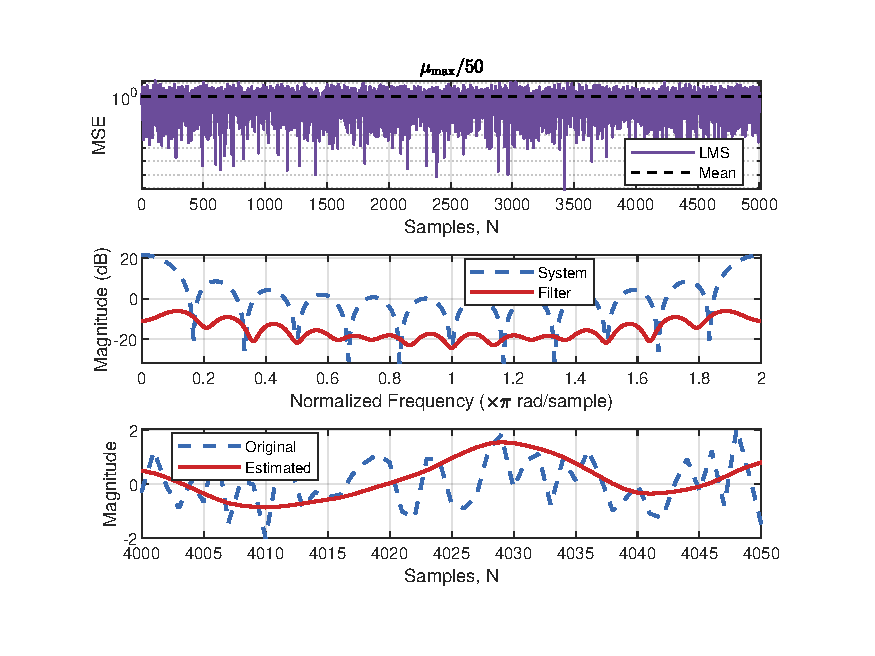
\includegraphics[width=0.9\textwidth]{C:/Users/lucasabdalah-dell/Documents/GitHub/Courses-HWs/Master/TIP7188-FILTRAGEM_ADAPTATIVA/homework/code/figures/hw3p5b-mu50.pdf}
    \caption{$\text{Amostras} = 5000$, $M = 15$, $\mu = \frac{\mu_{\text{max}}}{50}$}
    \label{fig:mu_50}
\end{figure}

\clearpage

\subsubsection*{Meça o desajuste (misadjustment)}
Para calcular o desajuste, podemos utilizar:
\begin{align*}
    M &= \frac{\xi_{\text{exc}}}{\xi_{\text{min}}} \\
    &\approx \frac{\mu \text{trace}(\mathbf{R}_{x})}{1 - \mu \text{trace}(\mathbf{R}_{x})}
\end{align*}

Utilizando o MATLAB, foi possível calcular o desajuste a partir dessa expressão foi possivel obter a Tabela~\ref{tab:desajuste}.

\begin{table}[!htp]
    \centering
    \begin{tabular}{|l|l|l|l|}
        \hline
        & $ \mu_{\text{max}}/2$ & $\mu_{\text{max}}/10$ & $\mu_{\text{max}}/50$ \\ \hline
        Téorico & -1.3846  & 2.5714 & 0.1682 \\ \hline
        Empírico & -1.3868 & 2.5342 & 0.1674 \\ \hline
    \end{tabular}
    \caption{Comparativo entre os valores de desajuste teóricos e empíricos.}
    \label{tab:desajuste}
\end{table}

\subsubsection*{Resposta em frequência do filtro FIR}
Já apresentado anteriormente nesta seção, a resposta em frequência do filtro é apresentada nas Figuras~\ref{fig:mu_2}, \ref{fig:mu_10} e \ref{fig:mu_50}. A resposta se assemelha muito do sistema que se deseja estimar para o caso de $\mu/2$. Pois o sistema tem mais adaptabilidade para seguir as mudanças do canal. Entretanto, se esse valor diminui, a identificação piora, tendo uma versão atenuadas do sistema em questão. Já para a análise no domínio do tempo, apenas o sinal do primeiro caso se assemelha, os outros dois sinais são bastante degradados e quase não se pode ver relação entre o original e o estimado.


\subsection{Equalização Adaptativa} % <-----------------------------------------------------------------------------


\subsubsection*{Treine o filtro adaptativo NLMS}

A evolução temporal do MSE apresenta comportamento similar aos problemas anteriores, com MSE tendo variação considerável até mesmo após a convergência, Figura~\ref{fig:hw3p6a-MSE}. Já na Figura~\ref{fig:hw3p6a-evolution}, observa-se a evolução temporal em quatro janelas de transmissão, permitindo a visualização dos símbolos enviados originalmente e de suas respectivas estimações.  Nos dois gráficos superiores, há a adaptação inicial do filtro, onde ainda há certa dificuldade para acompanhar a variação do canal. nas primeiras amostras. Nos dois inferiores, há janelas com etapas mais avançadas da adaptação, onde pode-se visulizar uma capacidade levemente superior de acompanhar o canal.

Além disso, é possível ver na figura~\ref{fig:hw3p6a-QAM} o impacto no filtro da aplicação da filtragem a um sinal de modução 16-QAM. A estimação visivelmente separa o sinal transmitido em diferentes regiões de decisão, que bastaria aplicar um decisor para reconstrução do sinal original modulado.


\clearpage

\begin{figure}[!htp]
    \centering
    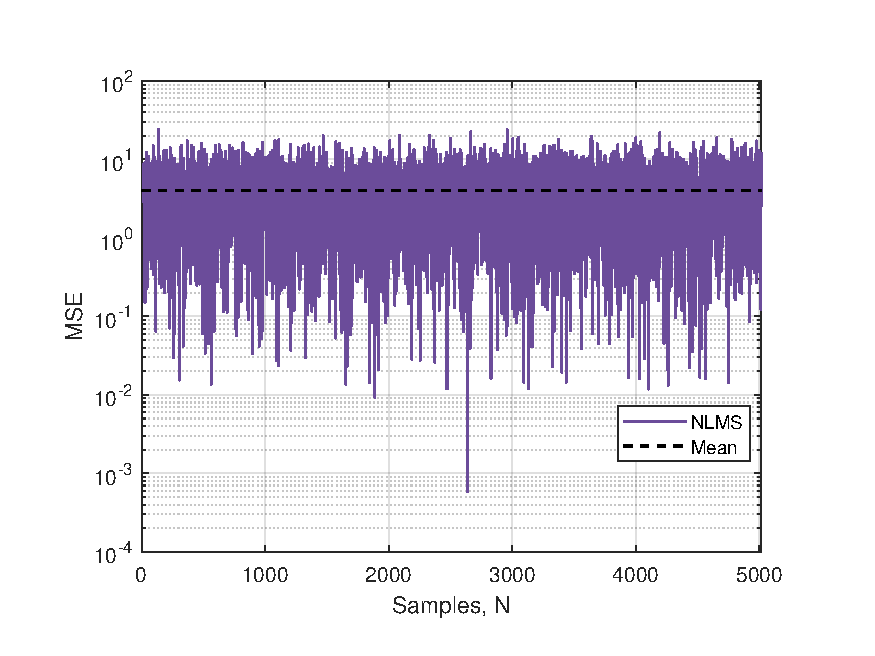
\includegraphics[width=0.8\textwidth]{C:/Users/lucasabdalah-dell/Documents/GitHub/Courses-HWs/Master/TIP7188-FILTRAGEM_ADAPTATIVA/homework/code/figures/hw3p6a-MSE.pdf}
    \caption{Curva de MSE para: $\text{Amostras} = 5000$, $M = 15$, $\mu = 0.4$.}
    \label{fig:hw3p6a-MSE}
\end{figure}

\begin{figure}[!htp]
    \centering
    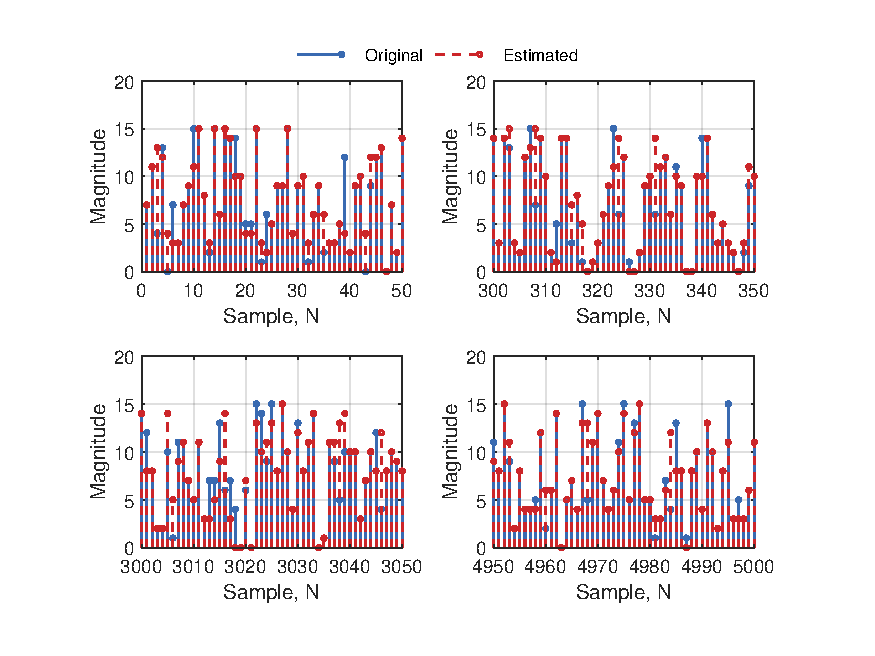
\includegraphics[width=0.8\textwidth]{C:/Users/lucasabdalah-dell/Documents/GitHub/Courses-HWs/Master/TIP7188-FILTRAGEM_ADAPTATIVA/homework/code/figures/hw3p6a-evolution.pdf}
    \caption{Evolução temporal: $\text{Amostras} = 5000$, $M = 15$, $\mu = 0.4$.}
    \label{fig:hw3p6a-evolution}
\end{figure}

\clearpage


\begin{figure}[!htp]
    \centering
    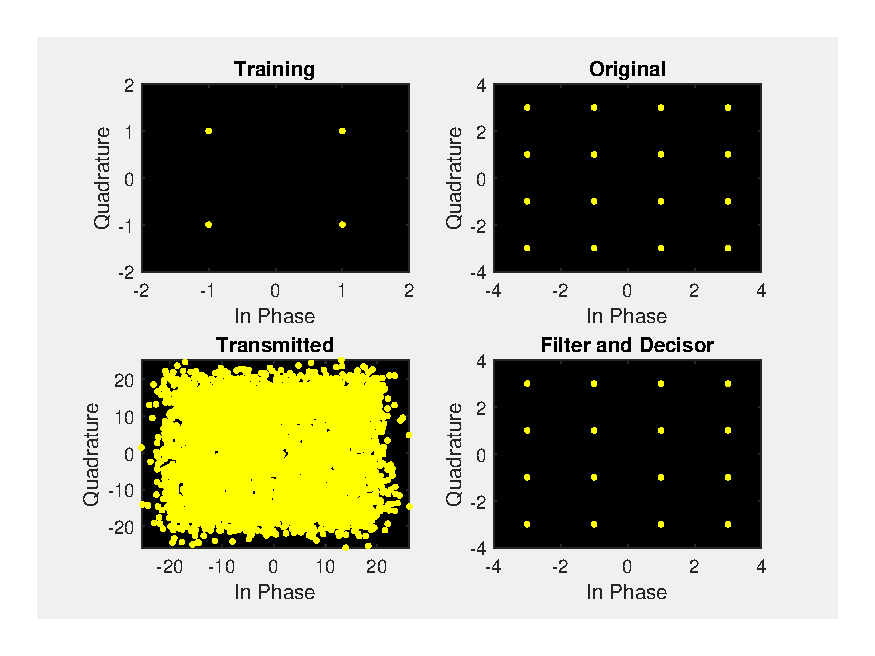
\includegraphics[width=0.7\textwidth]{C:/Users/lucasabdalah-dell/Documents/GitHub/Courses-HWs/Master/TIP7188-FILTRAGEM_ADAPTATIVA/homework/code/figures/hw3p6a-QAM.pdf}
    \caption{Esquema de Transmissão: $\text{Amostras} = 5000$, $M = 15$, $\mu = 0.4$.}
    \label{fig:hw3p6a-QAM}
\end{figure}

% \clearpage

\subsubsection*{Treine o filtro adaptativo LMS}
A variação do treino adaptativo de acordo com o número de amostras disposto na Figura~\ref{fig:hw3p6b-evolutionSamples}. Apenas por inspeção visual é uma tarefa complexa indicar comparações. Aparentemente, as variações entre as etapas diversas são bem sutis.

\begin{figure}[!htp]
    \centering
    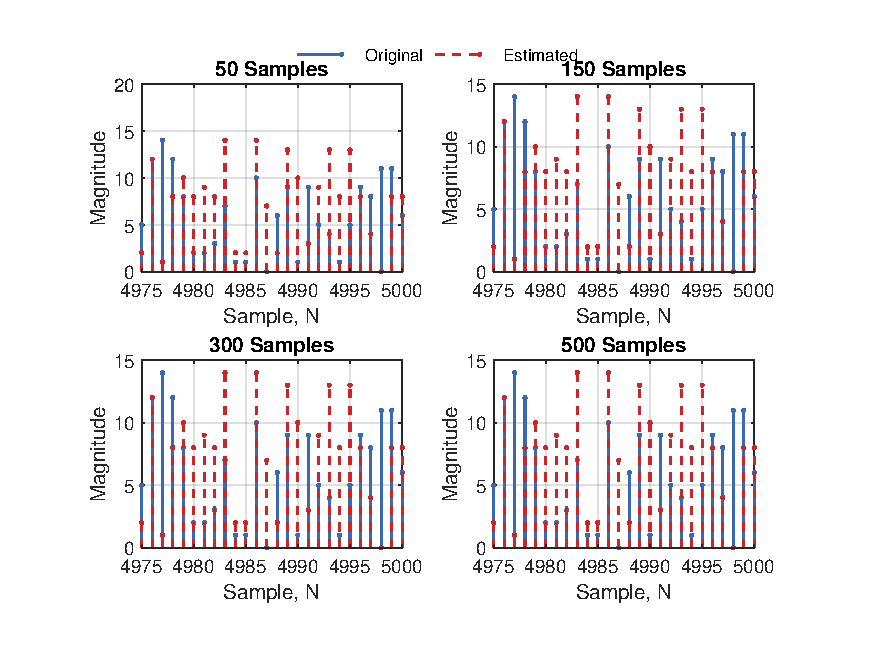
\includegraphics[width=0.7\textwidth]{C:/Users/lucasabdalah-dell/Documents/GitHub/Courses-HWs/Master/TIP7188-FILTRAGEM_ADAPTATIVA/homework/code/figures/hw3p6b-evolutionSamples.pdf}
    \caption{Evolução temporal de acordo com o tamanho da janela de treinamento: $\text{Amostras} = 5000$, $M = 15$, $\mu = 0.001$}
    \label{fig:hw3p6b-evolutionSamples}
\end{figure}

\clearpage

\subsubsection*{Dados transmitidos foram gerados de uma constelação 256-QAM}

\todo[inline, color=yellow!30]{Organizar}

A evolução temporal do MSE apresenta comportamento similar ao do primeiro problema. Entretanto, é notável que a média para a constelação 256-QAM é muito maior, o que segue o resultado esperado instintivamente, já que o espaço entre os símbolos é menor, provocando maior dificuldade da identificação do símbolo original. Além disso, o MSE apresenta variação considerável até mesmo após a convergência, Figura~\ref{fig:hw3p6c-MSE}. Já na Figura~\ref{fig:hw3p6c-evolution}, observa-se a evolução temporal em duas janelas de transmissão, permitindo a visualização dos símbolos enviados originalmente e de suas respectivas estimações.  No gráfico superior, há a adaptação inicial do filtro, onde ainda há certa dificuldade para acompanhar a variação do canal. nas primeiras amostras. Já no inferior, há uma etapas mais avançada da adaptação, onde pode-se visulizar uma capacidade levemente superior de acompanhar o canal.

Métricas de SER ou BER podem ajudar a identificar melhor problemas de adaptação do filtro para esse tipo de exercício.
    
\begin{figure}[!htp]
    \centering
    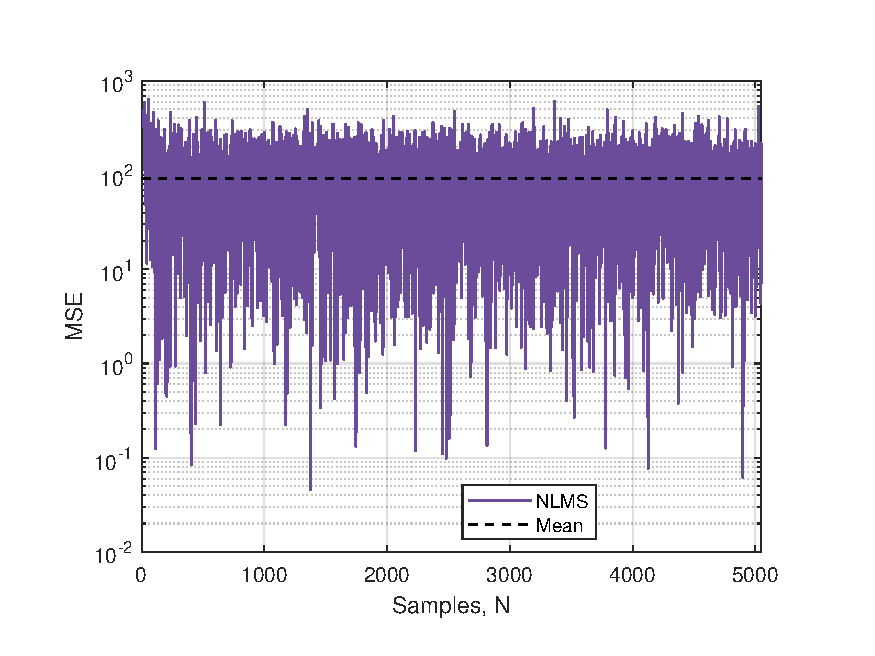
\includegraphics[width=0.9\textwidth]{C:/Users/lucasabdalah-dell/Documents/GitHub/Courses-HWs/Master/TIP7188-FILTRAGEM_ADAPTATIVA/homework/code/figures/hw3p6c-MSE.pdf}
    \caption{Curva MSE para: $\text{Amostras} = 5000$, $M = 15$, $\mu = 0.4$.}
    \label{fig:hw3p6c-MSE}
\end{figure}

\begin{figure}[!htp]
    \centering
    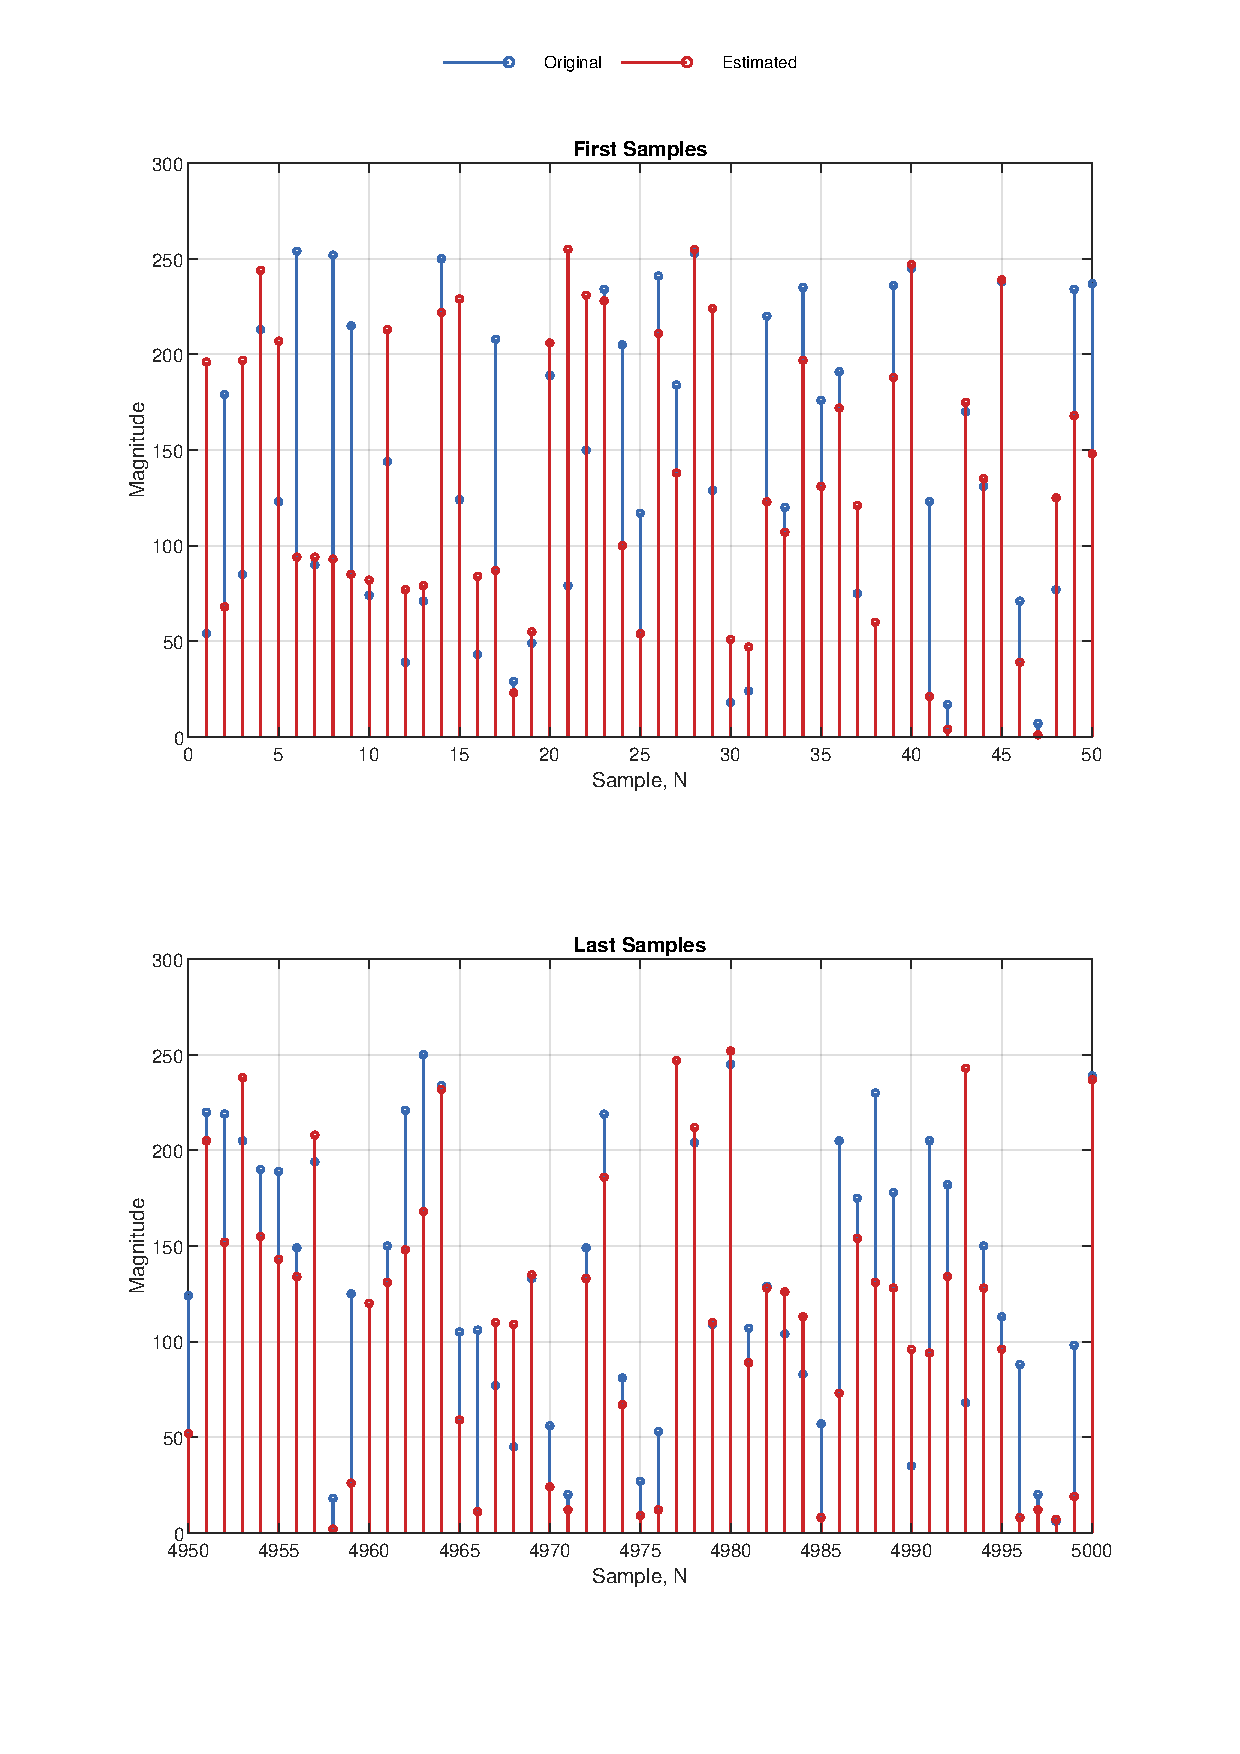
\includegraphics[width=0.9\textwidth]{C:/Users/lucasabdalah-dell/Documents/GitHub/Courses-HWs/Master/TIP7188-FILTRAGEM_ADAPTATIVA/homework/code/figures/hw3p6c-evolution.pdf}
    \caption{Evolução temporal: $\text{Amostras} = 5000$, $M = 15$, $\mu = 0.4$.}
    \label{fig:hw3p6c-evolution}
\end{figure}

\clearpage

\subsubsection*{Curvas de taxa de erro de símbolo (SER) versus SNR}
A Figura~\ref{fig:hw3p6d-SER} permite avaliar o real desempenho do filtro quando associado a um equalizador que desconhece o sinal verdadeiro.

Como esperado, é possível visualizar que ao passo que a ordem da modulação aumenta, o desempenho piora vertiginosamente. Isso está relacionado com o que já foi apresentado em seções anteriores, fenômeno decorrente da proximidade dos símbolos das constelações digitais, o que acarreta interferências de ruído do canal, aumentando a frequência dos erros de decisão.

Além disso, pode-se relacionar com o fator do treinamento, que utilizada uma constelação com apenas 4 símbolos e ao efetuar transmissões com esquema de modulação com até 64 vezes mais símbulos, apresenta um filtro de comprimento pequeno para compensar essa discrepância entre treino e transmissão.
    
\begin{figure}[!htp]
    \centering
    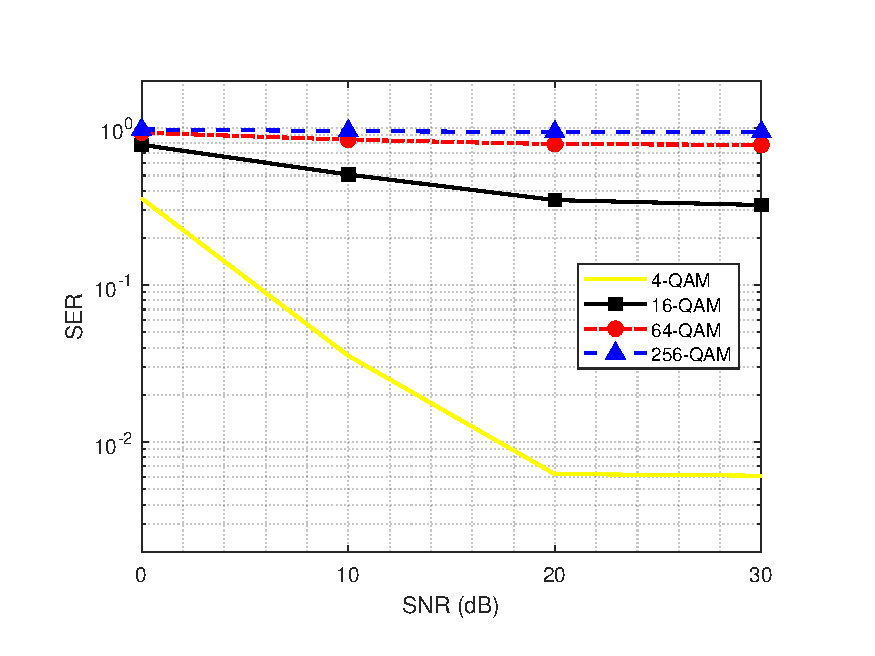
\includegraphics[width=0.9\textwidth]{C:/Users/lucasabdalah-dell/Documents/GitHub/Courses-HWs/Master/TIP7188-FILTRAGEM_ADAPTATIVA/homework/code/figures/hw3p6d-SER.pdf}
    \caption{SER vs SNR (dB) para 1000 realizações de Monte Carlo: $\text{Amostras} = 5000$, $M = 15$, $\mu = 0.4$}
    \label{fig:hw3p6d-SER}
\end{figure}
